\section{Designing \name}\label{s:design}
%
\cut{
\an{maybe move to ``bundler's utility regime''/Overview/``Traffic Bundles'': 
What is the best way to take advantage of the existence of traffic bundles?
Broadly, there are two approaches: congestion control and in-network scheduling. 
Today, congestion control is a distributed concern: each end-host performs its own optimization to achieve the highest throughput and lowest latency.
Indeed, end-host rate control is a deployed method to enforce domain-wide scheduling policy in private WANs~\cite{bwe}.
On the other hand, scheduling is an in-network concern; existing proposals such as DiffServ~\cite{diffserv} observe that the network is uniquely positioned to differentiate between different flows according to some domain-wide policy.
Scheduling presents its own challenge: because the Internet is a federated system, the link with queue build-up (and thus with the opportunity to re-order packets according to a scheduling policy) will likely be outside the sending domain's purview.

\an{don't know what to say next}
}
}

Recall that in order to do scheduling, we need to move the queues from the network to the \name. 
In this section, we first describe our key insight for moving the in-network queues, and then explain our specific design choices. 
Recall that each site deploys one \name middlebox which we logically partition into sender-side (\inbox) and receiver-side (\outbox) functionality.

\subsection{Key Insight}\label{s:design:key}
We induce queuing at the \inbox by rate limiting the outgoing traffic. 
If this rate limit is made smaller than the bundle's fair share of bandwidth at the bottleneck link in the network, it will decrease throughput. 
Conversely, if the rate is too high, packets will pass through the \inbox without queueing.
Instead, the rate needs to be set such that the bottleneck link sees a small queue while remaining fully utilized (and the bundled traffic competes fairly in the presence of cross traffic). 
We make a simple, but powerful, observation: existing congestion control algorithms calculate exactly this rate~\cite{Jacobson88}. 
Therefore, running such an algorithm to set a bundle's rate would reduce its self-inflicted queue at the bottleneck, causing packets to queue at the \inbox instead, without reducing the bundle's throughput.
Note that end hosts would continue running a traditional congestion control algorithm as before (\eg Cubic~\cite{cubic}, BBR~\cite{bbr}) which is unaware of \name.
Rather, the \inbox's congestion control algorithm acts on the traffic bundle as a \emph{single unit}.

Figure~\ref{fig:design:shift-bottleneck} illustrates this concept for a single flow traversing a bottleneck link in the 
network.\footnote{Details of the emulated network setup which resulted in the illustrated queue length time-series are in \S\ref{s:eval}.}
Without \name, packets from the end hosts are queued in the network, while the queue at the edge is unoccupied. 
In contrast, a \name deployed at the edge is able to shift the queue to its \inbox.

\subsection{System Overview}\label{s:design:overview}
\begin{figure}
    \centering
    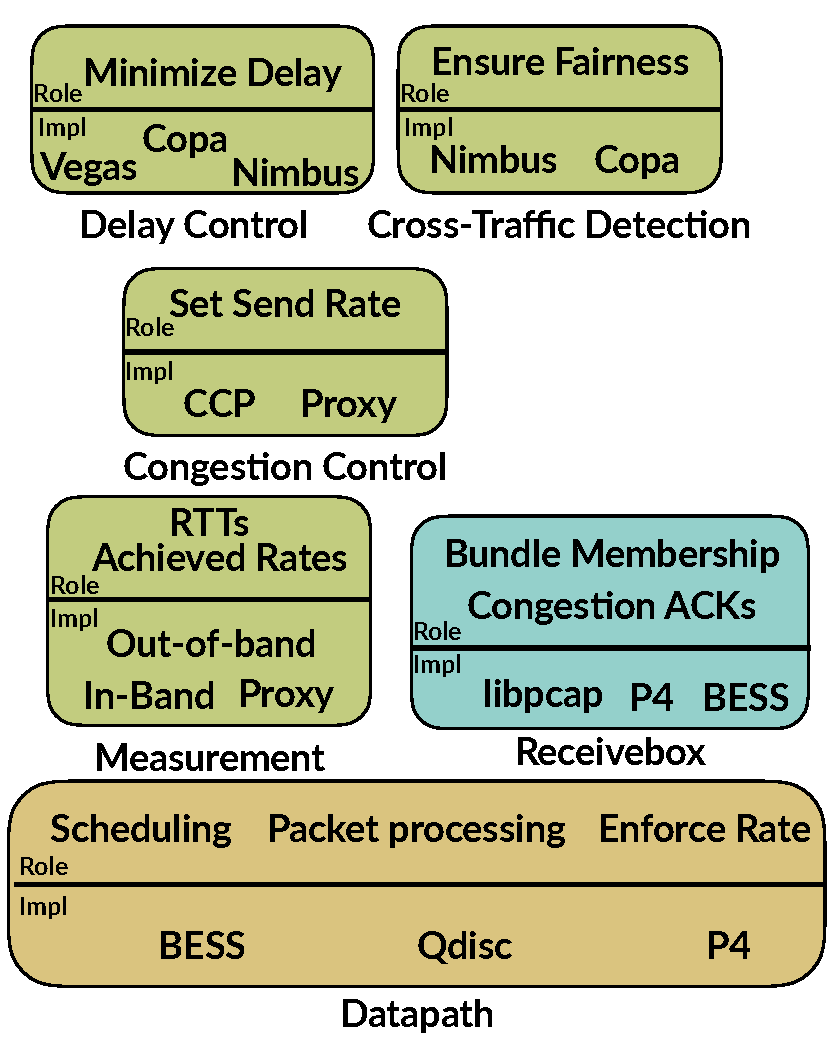
\includegraphics[width=\columnwidth]{img/arch-block-diag}
    \vspace{-40pt}
    \caption{\name comprises of six sub-systems: four (in green) implement \inbox functionality, one (in blue) implements \outbox functionality, and the datapath (orange) is shared between the two. \cut{\radhika{should we put the \name blocks inside another box called ``control plane''?}}}\label{fig:design:block-diag}
\end{figure}
%\fc{starts a bit abruptly, better lead in?}
% in order to run congestion control for an aggregation of flows, you need some way to measure the network. 
Figure~\ref{fig:design:block-diag} shows \name's sub-systems: 
(1) A congestion control module at the \inbox which implements the rate control logic and cross-traffic detection, as discussed in \S\ref{s:design:whichcc}.
(2) A mechanism for sending congestion feedback (ACKs) in the \outbox, and (3) a measurement module in the \inbox that computes congestion signals (RTT and receive rate) from the received feedback. We discuss options for implementing congestion feedback mechanism in \S\ref{s:design:twosided} and how to use that feedback in the measurement module in \S\ref{s:measurement}.
(4) A datapath for packet processing (which includes rate enforcement and packet scheduling). Any modern middlebox datapath, \eg BESS~\cite{bess}, P4~\cite{p4}, or  Linux qdiscs (as used in our prototype implementation---see \S\ref{s:impl}), is suitable. 
%\fc{should we add ecmp detection?} \radhika{can we think of it as part of measurement? let's not bring too much attention to it}
We detail the interaction between these subsystems when discussing our prototype implementation in \S\ref{s:impl}. 
%
%\an{radhika, pls check this subsection and the figure. I think it no longer requires understanding how everything works and is more of an overview?}
%\radhika{i think it looks good now! i edited it slightly -- adding more detailed sentences so that it gives a slightly more holistic overview. please check. Also, do you want to update fig 5 to make it even more consistent with this? e.g. in Fig 5, replace `Send Box' with `Measurement', `Receive box' with `Congestion ACKs', `CCP' with `Congestion Control (CCP)'? You can have the terms SendBox and ReceiveBox outside the boxes.}
%Figure~\ref{fig:design:block-diag} shows the necessary components of \name: (1) a means of determining bundle membership; (2) a rate enforcement mechanism; (3) a measurement strategy; (4) a delay-controller; and (5) a fairness-controller.
%Throughout this section we discuss design options for determining Bundle membership (\S\ref{s:design:membership}), observing feedback (\S\ref{s:design:twosided}), and congestion control (\S\ref{s:design:whichcc}): for other aspects of the design, \name is compatible with a variety of options. For example, domains can implement \name using any modern middlebox datapath, \eg P4~\cite{p4}, BESS~\cite{bess}, or as in our prototype implementation (\S\ref{s:impl}), Linux tc qdiscs.
%\radhika{maybe we can chop this subsection off -- let's discuss.}
%
In the rest of this section, we discuss our key design choices.
%Our overarching design principle is simplicity; at various points in the design, there exists a more complex approach which we discard.\fc{why? maybe just remove this?} \radhika{yes, can remove}

\cut{
\subsection{Identifying Bundle Membership}\label{s:design:membership}
\an{I think we can cut this with the site-to-site framing.}
\name must first identify which packets (or flows) are part of the same traffic bundle.
To compute and enforce correct sending rates for a traffic bundle, it is important to only bundle those flows that share the same bottleneck.
%; otherwise, \name may send a component flow at the wrong rate for its bottleneck.
This has traditionally been a difficult problem; 
Rubenstein \etal~\cite{active-sharedbottlenecks} use a ``poisson-probing'' mechanism to probabilistically identify shared bottlenecks under a limited network model, and
multipath TCP~\cite{mptcp} sidesteps it with a weighted window increase-decrease protocol.

Deploying \name boxes close to both endpoints allows us to adopt a more direct (and accurate) approach based on a \emph{two-way opt-in}.
In this approach, a site must agree to bundle traffic on both the sending and receiving sides.
The first step, of course, is to place a \name middlebox at the domain's edge.
Initially, the \inbox assumes all component traffic is unbundled.
When the \outbox observes an unbundled packet, it opts-in by sending an initialization message
\footnote{To avoid sending an initialization message for every unbundled packet, the \outbox samples the unbundled packets using the same mechanism as in \S\ref{s:measurement}.} 
(analogous to TCP's SYN) 
containing the IP prefixes it covers, addressed to the source IP of the packet
\footnote{Addressing to the source IP of the packet is not strictly necessary; domains may also advertise \inbox{}es via \eg DNS.}.
If there is no \inbox on the path, this message will be ignored.
Otherwise, a \inbox will observe this message and can opt-in by initializing a new traffic bundle corresponding to the \outbox's destination prefixes and sending a message (analogous to TCP's SYNACK) notifying the \outbox of the source IP prefixes it covers, so the \outbox can initialize a bundle corresponding to that sending domain.
Now, the \inbox and \outbox can identify packets belonging to initialized bundles by matching the corresponding IP prefixes.
Any subsequent packets the \outbox observes from that sending domain are treated as part of the bundle.

%The \outbox does one of two things for each potential epoch boundary packet:
%\begin{enumerate}
%    \item If the packet is in a known bundle, the \outbox sends a message to the corresponding \inbox.
%    \item If the packet is not in a known bundle, the \outbox sends a message to the source IP address of that packet.
%\end{enumerate}

%The \inbox receives (and intercepts) the \outbox feedback.  
%The \inbox at this time updates its flow tables to add the destination IP of the epoch boundary packet either to an existing bundle (in the case of a new flow from a previously-unseen source subnet joining a bundle) or instantiates a new bundle.
%The \inbox then sends a response containing an epoch size to use and the hash of the epoch boundary packet.
%The \outbox receives this message, initializes a byte counter for the newly discovered bundle, and remembers the \inbox IP address for future feedback. If there is no \inbox on the path, the packet will simply be ignored at its destination. 
}

\subsection{Choice of congestion control algorithm}\label{s:design:whichcc}
\name's congestion control algorithm must satisfy the following requirements: 

\paragraphi{(1) Ability to limit network queueing} \name must limit queueing in the network to move the queues to the \inbox. Therefore, congestion control algorithms which are designed to control delays, and thus queueing, are the appropriate choice. 
A loss-based congestion control algorithm which fills buffers (\eg Cubic, NewReno), for example, is not a good choice for \name, since it would build up a queue at the network bottleneck and drain queues at the \inbox.

\paragraphi{(2) Detection of buffer-filling cross-traffic} It is well known that delay-controlling schemes (\eg Vegas~\cite{vegas}) compete poorly with buffer-filling loss-based schemes~\cite{copa}.
Therefore, \name must have a mechanism to detect the presence of such competing buffer-filling flows and fall back to status quo performance, and then detect when they have left to take back its control over the network queues. 

The emergence of such detection mechanisms is recent: Copa~\cite{copa} detects whether it is able to empty the queues, and Nimbus~\cite{nimbus-arxiv} provides a more general mechanism which overlays a pattern on the sending rate and measures the cross traffic's response.
Copa is not designed for aggregate congestion control (see \S\ref{s:queue-ctl}); thus, we use the more general Nimbus mechanism.

\subsection{Congestion Feedback Mechanism}\label{s:design:twosided}
A congestion control algorithm at the \inbox would require network feedback from the receivers to measure congestion and adjust the sending rates accordingly. We discuss multiple options for obtaining this. 

%This problem presents multiple possible solutions:

\paragrapha{Passively observe in-band TCP acknowledgements}
Conventional endhost-based implementations have used TCP acknowledgements to gather congestion control measurements. A simple strategy for \name is to passively observe the receiver generated TCP acknowledgements at the \inbox. However, we discard this option as it is specific to TCP and thus incompatible with alternate protocols, \ie UDP for video streaming or QUIC's encrypted transport header~\cite{quic}.

\paragrapha{Terminate connections and proxy through TCP} With this approach, one would terminate end-host TCP connections at the \inbox and open new connections to the \outbox, allowing the \inbox to control the rate of traffic in these connections.
%This approach allows the unmodified use of existing congestion control algorithms for the TCP connection between the \inbox and the \outbox \radhika{edited, pls check}. 
%since a TCP tunnel can collect ACKs. 
This approach can improve performance by allowing end-to-end connections to ramp up their sending rates quickly. 
%\radhika{unclear} \radhika{also, wouldn't this approach have the same disadvantage as previous one?}
The primary disadvantage of this approach is that \name must take responsibility for reliable delivery of component traffic, which requires large amounts of queueing and, in the case of UDP applications, can harm application performance. 
Furthermore, proxying TCP connections introduces a new potential point of failure at \name that violates fate-sharing; if \name crashes, connections will be lost.
Finally, from a practical standpoint, to avoid head-of-line blocking this approach requires that \name open a new proxy connection for each component end-host connection, but still determine the bottleneck rate of the traffic \emph{aggregate}. While this approach may be technically feasible~\cite{cm}, it would result in high overhead.
\cut{\footnote{From an architectural standpoint this design runs counter to the end-to-end principle~\cite{e2e-principle}; it replicates endhost functionality in the network.}}
%the cycles used for opening and managing new proxy connections are better used for packet processing.
Thus, we set aside TCP proxies for the remainder of this discussion, but explore their compatibility with \name in \S\ref{s:eval:proxy}. 
%We but note that this approach is complementary with \name (see \S\ref{s:eval}).

%\an{discuss non-terminating tcp tunnels?}
\paragrapha{Out-of-band feedback} Having eliminated the options for using in-band feedback, we adopt an out-of-band feedback mechanism: the \outbox sends out-of-band congestion ACKs to the \inbox.
This decouples congestion signalling from traditional ACKs used for reliability\footnote{The idea of an out-of-band congestion notification is similar to that in QCN~\cite{qcn}, although our goals differ.} and is thus indifferent to the underlying protocol (be it TCP, UDP, or QUIC).
%We detail the congestion measurement strategy and contents of congestion ACKs in \S\ref{s:measurement}.

\cut{
\begin{Appendix}
\section{Nimbus}\label{s:app:nimbus}
\begin{figure*}[ht!]
    \centering
\begin{knitrout}
\definecolor{shadecolor}{rgb}{0.969, 0.969, 0.969}\color{fgcolor}
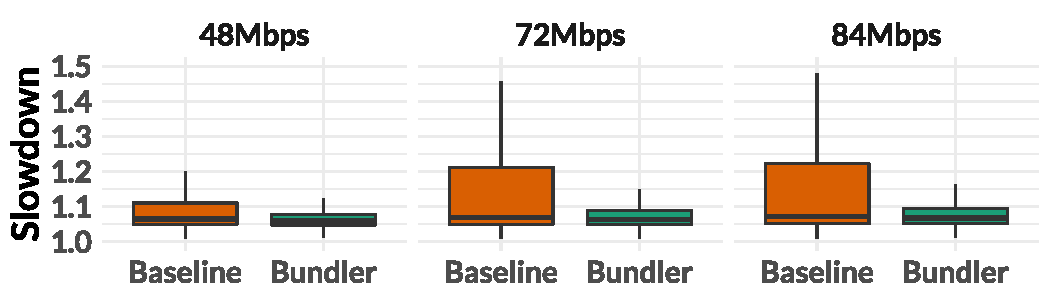
\includegraphics[width=\maxwidth]{figure/eval:offeredload-1} 

\end{knitrout}
    \caption{\name offers diminishing returns with lower amounts of offered load.}
    \label{fig:eval:offeredload}
\end{figure*}
%
%\newcommand{\highUtilTailImprove}{round(highUtilTailImprove, 0)\%\xspace}
%\newcommand{\medUtilTailImprove}{round(medUtilTailImprove, 0)\%\xspace}
%\newcommand{\lowUtilTailImprove}{round(lowUtilTailImprove, 0)\%\xspace}


We briefly summarize Nimbus~\cite{nimbus} for reference.

Nimbus's goal is to detect scenarios in which it is safe to use delay-based congestion control. 
To achieve this goal, Nimbus proposes an \emph{elasticity detector} to detect whether the cross traffic contains any \emph{elastic} flows, which react to changes in the available bandwidth on fast time-scales, \ie a couple RTTs. 
Nimbus's core observation is that the absence of such elastic cross traffic, \ie competition with only \emph{inelastic} traffic, is a sufficient (but not necessary) condition to use a delay-control algorithm.
Nimbus thus measures whether cross traffic reacts to changes in available bandwidth by pulsing its sending rate at a predetermined frequency.
If the cross traffic's rate responds to these pulses at the same frequency, Nimbus can conclude that it is elastic, because it has reacted to changes in the available bandwidth.

A natural method of measuring the cross traffic's frequency response is to compare Nimbus's pulses with the cross traffic's rate in the frequency domain.
Thus, Nimbus uses an asymmetric sinusoidal pulse (as we have noted in \S\ref{s:queue-ctl}) which has a straightforward representation in the frequency domain while maximizing the sender's ability to influence the available bandwidth.

How can Nimbus know the cross traffic's response? It develops an estimator for the cross traffic's sending rate:
\begin{equation}
    \hat{z}(t) = \mu\frac{S(t)}{R(t)} - S(t)
\end{equation}

$\hat{z}(t)i$ is the estimated cross traffic rate, $\mu$ is the estimated bottleneck bandwidth, $S(t)$ is the sending rate, and $R(t)$ is the receiving rate. 
    \name measures $R(t)$ using congestion ACKs from the \outbox and $\mu$ using the maximum receive rate as in BBR~\cite{bbr}.

Then, Nimbus searches for a peak in the neighborhood of its pulsing frequency $f_p$ to determine the elasticity metric $\eta$:

\begin{equation}
    \eta = \frac{|\text{FFT}_{\hat{z}}(f_p)|}{\text{max}_{f \in (f_p, 2f_p)} |\text{FFT}_{\hat{z}}(f)|}
\end{equation}

If $\eta$ is larger, the cross traffic is more elastic.
Nimbus then uses a hard-decision rule $\eta \ge 2$ to decide when to switch to cross-traffic competitive mode as described in \S\ref{s:queue-ctl}.

\end{Appendix}
}

\section{Measurement Strategy}\label{s:measurement}

In this section we describe how the \inbox and \outbox coordinate to compute accurate and robust
measurements of the network conditions necessary as inputs to congestion control algorithms.

Congestion control algorithms need only a small, common set of measurements~\cite{ccp-hotnets}. 
In particular, rate-based algorithms need only three measurements: 
the sending rate, receiving rate, and path round-trip time.
A significant complication is that for accurate measurements on RTT time-scales, we must calculate send and receive rates over the same set of packets~\cite{packettrain}.
This requirement drives the design of our measurement methodology.

\subsection{Determining Epoch Boundary Packets}
\label{s:measure:marking}
Consider the stream of packets $P_B$ from all flows in a bundle $B$ in the order they leave the \inbox after scheduling.
The \inbox and \outbox need to know how to divide this stream into sets 
of packets --- which we call \emph{epochs} --- over which they can calculate measurements.
For now, we make the simplifying assumption that packets arrive at the \outbox in the same order they 
left the \inbox (we address re-ordering in Section~\ref{s:measure:limitation:reorder}). \an{note about re-ordering is a little distracting and doesn't help explain approach}
This simplifies the problem into deciding, for all given packets in $P_B$, whether it is an epoch boundary packet at which the current epoch should end and the next should begin. 
Suppose for now that we wish to have a fixed epoch size of $N$ packets.
A naive approach would be to mark the boundary between epochs every $N$ packets. 
However, this strategy is brittle; a single lost packet would de-synchronize the boxes' views of the epochs. 
More generally, any strategy that requires packet-level synchronization of the \inbox and
\outbox is untenable because any coordination would race the packets themselves.

The key idea of our methodology is that we can avoid such a synchronization problem by determining the boundary of an epoch using only information contained in the packet.
Specifically, we propose the following: a packet $p$ is an epoch boundary packet if the hash 
of some subset of its header (see below) modulo the epoch size $N$ is equal to 0, that is:
$$B(p,N) \coloneqq H(p)\ \text{mod}\ N == 0$$
Thus, an epoch boundary packet will occur (in expectation) once every $N$ packets.
For $H$, we use the Fowler/Noll/Vo (FNV) hash function~\cite{fnv-hash}, a non-cryptographic fast hash function with a low collision rate. 

\paragrapha{Choosing header subset} The header subset we use must remain constant as the packet traverses the network from the \inbox to the \outbox; otherwise, they would not be able to agree on epoch boundaries. This rules out simple approaches such as hashing the entire packet header, since the TTL field will decrement between the inbox and outbox.
Even the 5-tuple of the packet may change, since the outbox may be behind a NAT.
Using TCP sequence numbers is tempting, but retransmissions may confuse RTT measurements.

We use the IP ID field, which will change every packet. This is an imperfect solution, as modern NATs may rewrite the IP ID field~\cite{ipid}.
Ultimately, the appropriate field to use will depend on the specific deployment of \name.

\subsection{Computing Measurements}
\label{s:measure:compute}
\newcommand{\pone}{$p_{prev}$}
\newcommand{\hpone}{$h(p_{prev})$}
\newcommand{\sone}{$s_{prev}$}
\newcommand{\rone}{$r_{prev}$}
\newcommand{\ptwo}{$p_{curr}$}
\newcommand{\hptwo}{$h(p_{curr})$}
\newcommand{\stwo}{$s_{curr}$}
\newcommand{\rtwo}{$r_{curr}$}
\newcommand{\atwo}{$a_{curr}$}
\newcommand{\sentone}{$sent_{prev}$}
\newcommand{\recvdone}{$rcvd_{prev}$}
\newcommand{\senttwo}{$sent_{curr}$}
\newcommand{\recvdtwo}{$rcvd_{curr}$}


\begin{figure}
    \centering
    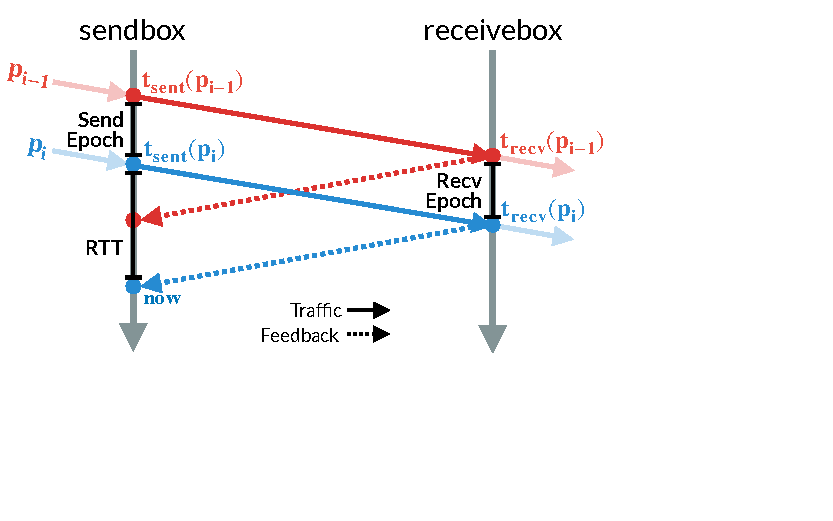
\includegraphics[width=\columnwidth]{img/rate-calculation}
    \caption{Example of epoch-based measurement calculation. Time moves from top to bottom.
    Packets from flows in a bundle
    pass through the \inbox and \outbox middleboxes on the way to their destination. When 
    the inbox observes a packet header matching the boundary condition, it records it. When
    the \outbox observes such a packet, it sends an out-of-band feedback message back to
    the \inbox, which allows it to calculate the RTT and epochs.}\label{fig:ratecalc}
\end{figure}

Given this method of marking epochs, we can now construct the procedure for computing measurements.

For a given bundle, the \inbox runs the aforementioned function on each packet $p$. Each time
the function returns true, the \inbox updates an epoch data structure that records the packet hash,
which we will call \hptwo\ for the current epoch, 
along with the current time \stwo\ and the \emph{cumulative} number of bytes sent so far, \senttwo. This structure
is sorted by the time the packet was sent, \stwo, but is indexable by the packet hash.

The \outbox runs the same function. Each time it observes a boundary packet, 
it immediately sends a feedback message to the \inbox containing the same information:
the packet hash \hptwo, the time at which it received the packet, \rtwo, and the cumulative number of bytes
\emph{received} up until that point. When the \inbox receives this feedback message at time \atwo, it looks up the
packet hash \hptwo\ in the epoch data structure, which represents the end of the current epoch,
along with the earliest boundary packet still in the data structure, \hpone\ which represents the start
of the current epoch. It now has all of the information necessary to calculate one sample of the following:
\begin{subequations}
    \begin{align}
        RTT &= &now - s_2 \\
        send\_epoch\_duration &= &s_2 - s_1\\
        recv\_epoch\_duration &= &r_2 - r_1\\
        bytes\_sent\_in\_epoch &= &bytes\_sent\ at\ s_2 &\ - \\
                                    &&bytes\_sent\ at\ s_1&\notag\\
        bytes\_rcvd\_in\_epoch &= &bytes\_rcvd\ at\ r_2 &\ - \\
                                &&bytes\_rcvd\ at\ r_1\notag\\
        send\_rate &= &\frac{bytes\_sent\_in\_epoch}{send\_epoch\_duration}\\
        recv\_rate &= &\frac{bytes\_rcvd\_in\_epoch}{recv\_epoch\_duration}
    \end{align}
\end{subequations}
%(Note $bytes\_rcvd\_in\_epoch$ can also be interpreted as the number of bytes
%acknowledged for that epoch, which is a common signal used by many conestion
%control algorithms.)
Finally, it clears all marked packets preceding \ptwo\ leaving \ptwo\
to be the start of the next epoch.

\subsection{Fault Tolerance}
\label{s:measure:loss}
\paragrapha{Packet loss} This method is robust to the loss of boundary packets between the \inbox and \outbox.
Suppose the \inbox sees boundary packets $p_1, p_2, p_3$, but $p_2$ is lost after passing through
the \inbox so the \inbox only receives feedback for $p_1$ and $p_3$. Upon receiving $p_1$, 
the \inbox will truncate its data structure up until $p_1$. Upon receiving $p_3$, the \inbox 
looks up the oldest remaining boundary packet, $p_1$, and considers that the beginning of the epoch.
As a result, the epoch is longer than expected, but no measurements are lost or corrupted. 
The same argument applies to the loss of feedback messages. 
Importantly, \inbox calculates both the send and receive epoch based on information
from the \outbox rather than attempting to reach consensus on individual epoch boundaries with the \outbox. 

\paragrapha{Crashes \an{need better heading}} Existing work~\cite{ftmb} has studied how to design stateful middleboxes to be fault-tolerant with acceptable performance overheads. 
However, state-persistence is largely unnecessary for \name.
\name only stores network conditions, which it can re-learn within a few RTTs, and bundle membership flow tables, which it can re-discover as we describe in~\S\ref{s:impl:discovery}. 

\subsection{Choosing The Epoch Size}
\label{s:measure:epoch}
How do we choose the number of packets that should be in each epoch?
In 3.1, we assumed a fixed epoch size of $N$ packets.
However, in practice, the epoch must be a function of the sending rate.
If the epoch size is too small relative to the rate,
the epochs will be easily influenced by bursts and thus the measurements will be highly variable
and not useful.
If the epoch size is too large relative to the rate, the congestion control algorithm will not
receive feedback frequently enough to respond promptly to changing network conditions. 
As shown in prior work, congestion control algorithms can behave properly even if their
signals are only updated roughly once per RTT~\cite{ccp-hotnets}.
Setting the epoch size equal to our estimate of the number of packets currently inflight 
(our current sending rate multipled by our current esimate of the RTT) will yield roughly
one epoch and thus a new set of measurements per RTT.

Since the rate and thus the number of inflight packets is continuously changing over time,
we need to continually update the epoch size. Rather than using exactly the number of inflight
bytes, we round the value down to the nearest power of two so that the new epoch size is
always a multiple of the old one and thus will be compatible. 

For examaple, \fc{is an example necessary?}
if the inbox is marking every 256 packets
and the \outbox is marking every 512 packets, 
the inbox is just marking a super set of the \outbox packets, 
so it is effectively equivalent to them both marking every 512 packets.

\fc{Add explanation of windows}.
    
\subsection{Microbenchmarks}
\label{s:measure:microbench}
    \begin{figure}
    \centering
\begin{knitrout}
\definecolor{shadecolor}{rgb}{0.969, 0.969, 0.969}\color{fgcolor}
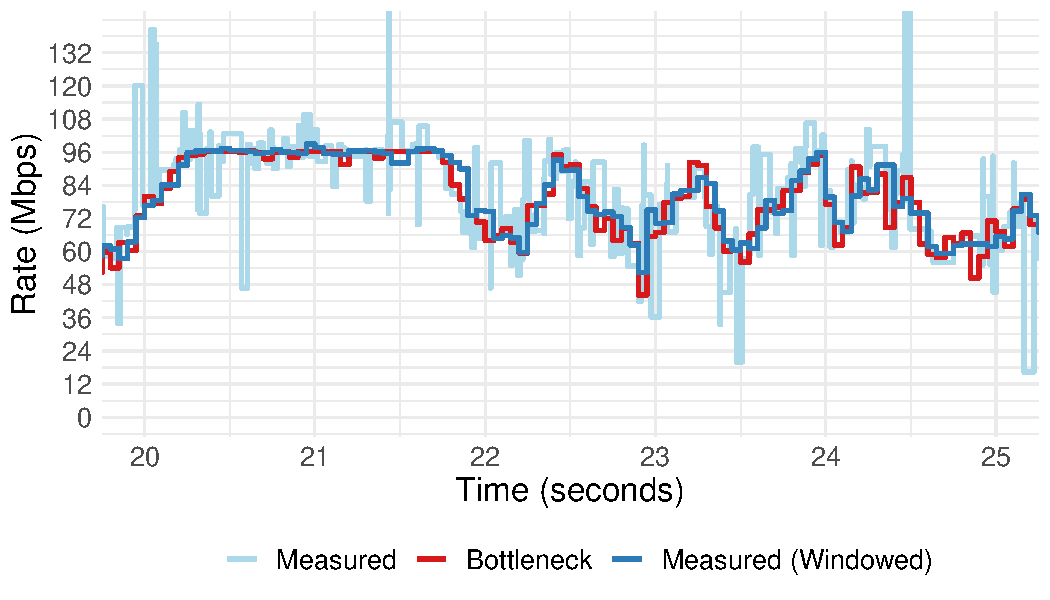
\includegraphics[width=\maxwidth]{figure/micro:time-1} 

\end{knitrout}
    \caption{\name's estimate of the receive rate compared to the actual rate leaving the bottleneck over a five second trace. 
    \name's raw estimate of the rate hovers around the true value, but is noisy. Averaging over a window of previous epochs
    yields a much smoother estimate that closely matches the true value.}
    \label{fig:micro:time}
\end{figure}

    \begin{figure}
    \centering
\begin{knitrout}
\definecolor{shadecolor}{rgb}{0.969, 0.969, 0.969}\color{fgcolor}
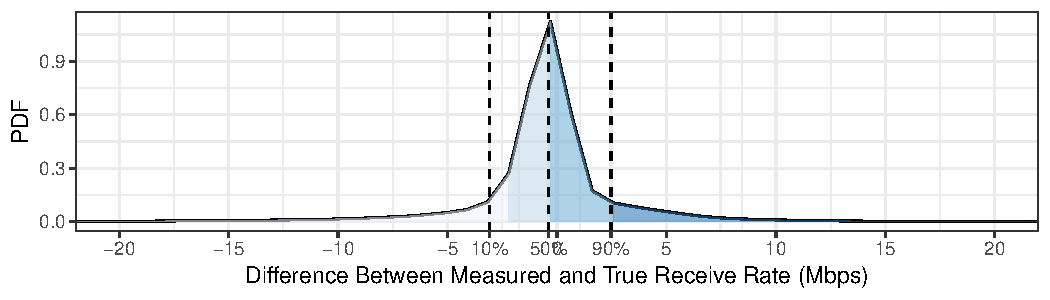
\includegraphics[width=\maxwidth]{figure/micro:thru-1} 

\end{knitrout}
    \caption{Distribution of the difference between \name's smoothed estimate of the receive rate and 
    the true bottleneck rate at each time point across all experiments. In most cases, the difference
    is negligble.}
    \label{fig:micro:thru}
\end{figure}

    \begin{figure}
    \centering
\begin{knitrout}
\definecolor{shadecolor}{rgb}{0.969, 0.969, 0.969}\color{fgcolor}
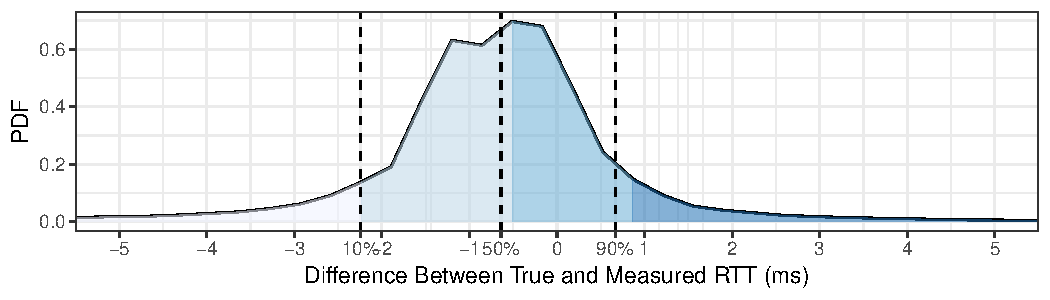
\includegraphics[width=\maxwidth]{figure/micro:delay-1} 

\end{knitrout}
    \caption{Distribution of the difference between \name's smoothed estimate of the RTT and 
    the true RTT (based on the queueing delay at the bottleneck router) at each time point across all experiments. In most cases, the difference
    is negligble.}
    \label{fig:micro:delay}
\end{figure}

    In this section we explore how well our measurements match the actual network conditions. 

    First, we consider our estimate of the receive rate (via Equation 1g). In Figure~\ref{fig:micro:time}
    we compare our esimate of the receive rate (``Measured'') to the actual rate of packets 
    leaving the bottleneck over a five second segment from one run in our evaluation (\fc{expand}).
    Here we demonstrate the necessity of a window to smooth out the estimation.

    In Figure~\ref{fig:micro:thru}, we compute the difference between our smoothed estimate of the receive rate 
    and the bottleneck rate at each time step and plot the distribution of this difference across
    all of the traces in our evaluation. 80\% of the time our estimate is within 3Mbps of the 
    actual rate.

    In Figure~\ref{fig:micro:delay}, we compute the difference between our estimate of the RTT between
    the \inbox and \outbox and the actual RTT at each time stpe and plot the distribution again
    across all of the traces in our evaluation. 80\% of the time we are within 2ms of the actual RTT.
    
\subsection{Limitations}
\subsubsection{Re-Ordering}
\label{s:measure:limitation:reorder}
Earlier we ignored re-ordering of packets between the \inbox and \outbox. However, if packets
are re-ordered, the \inbox and \outbox will observe a different view of the same epoch.
For example, consider packets numbered 1 to 20, where 10 is a boundary packet. The \inbox observes
10 packets in each epoch: [1,10] in epoch 1 and [11,20] in epoch 2. 
However, suppose packet 7 is delayed and arrives after packet 10. The \outbox will observe 9
packets in epoch 1 and 11 packets in epoch 2. 
Spurious re-ordering can be compensated by using an EWMA across epochs rather than the raw values
calculated at each epoch. If there is persitent re-ordering, it may be necessary to add a constant 
value to either the send or receive rate to compensate.

\subsubsection{Suitable Algorithms}
\label{s:measure:limitation:algs}
The set of measurements we obtain are sufficient for most rate-based algorithms, but may not be 
suitable for traditional window-based algorithms which require low-level metrics such as 
the number of inflight packets or number of packets lost. Although it should be possible
to compute these from the measurements we already collect in an ideal scenario, they would easily
break in the presence of network anomilies such as re-ordering. Thus, we leave the development
of robust signals for window-based algorithms to fuure work. 
Thus, \name currently operates best with rate-based algorithms such as BBR, Nimbus, or Copa~\cite{bbr,nimbus,copa}.


\subsection{Implications of \name's Design}

Our design choices result in an architecture where \name's inner rate control loop can be implemented entirely the ``control plane'' of the \inbox and the \outbox, which passively observes the packets traversing the datapath of the middleboxes, without modifying them. This results in a truly transparent system, that is light-weight, has low overhead, preserves fate-sharing, and in no way interferes with the end-to-end controllers of individual flows. The only datapath action that \name performs is the enforcement of the desired scheduling and queue management policies at the \inbox. 
%\radhika{added this subsection, since i think we weren't emphasizing on this enough. feel free to cut if running out of space.}